\documentclass{article}
\usepackage[utf8]{inputenc}
\usepackage{tikz}

% Importación de librerías
\usepackage{geometry}                   % Dimensiones y geometría del documento
\usetikzlibrary{shapes.geometric, arrows}
\tikzstyle{startstop} = [rectangle, rounded corners, minimum width=3cm, minimum height=1cm,text centered, draw=black]
\tikzstyle{io} = [trapezium, trapezium left angle=70, trapezium right angle=110, minimum width=3cm, minimum height=1cm, text centered, draw=black, fill=blue!30]
\tikzstyle{process} = [rectangle, minimum width=3cm, minimum height=1cm, text centered, text width=3cm, draw=black, fill=orange!30]
\tikzstyle{decision} = [diamond, minimum width=2cm, minimum height=1cm, text centered, draw=black, fill=green!30]
\tikzstyle{arrow} = [thick,->,>=stealth]

% Configuración página
\newcommand{\defaultpagemarginleft}{1}          % Margen izquierdo de las páginas [cm]
\newcommand{\defaultpagemarginright}{1}         % Margen derecho de las páginas [cm]
\newcommand{\defaultpagemargintop}{1}           % Margen superior de las páginas [cm]
\newcommand{\defaultpagemarginbottom}{1}        % Margen inferior de las páginas [cm]

% Definición de funciones
\newcommand{\lpow}[2]{{#1}_{#2}}          % Insertar sub-índice
\newcommand{\pow}[2]{{#1}^{#2}}           % Insertar elevado
\newcommand{\fracpartial}[2]{             % Fracción de derivadas parciales af/ax
	\frac{\partial #1}{\partial #2}}
\newcommand{\fracdpartial}[2]{            % Fracción de derivadas parciales dobles a^2/ax^2
	\frac{{\partial}^{2} #1}{\partial {#2}^{2}}}
\newcommand{\fracnpartial}[3]{            % Fracción de derivadas parciales en n a^n/ax^n
	\frac{{\partial}^{#3} #1}{\partial {#2}^{#3}}}
\newcommand{\fracderivat}[2]{             % Fracción de derivadas df/dx
	\frac{\text{d} #1}{\text{d} #2}}
\newcommand{\fracdderivat}[2]{            % Fracción de derivadas dobles d^2/dx^2
	\frac{{\text{d}}^{2} #1}{\text{d} {#2}^{2}}}
\newcommand{\fracnderivat}[3]{            % Fracción de derivadas en n d^n/dx^n
	\frac{{\text{d}}^{#3} #1}{\text{d} {#2}^{#3}}}
\newcommand{\topequal}[2]{                % Llave superior de equivalencia
	\overbrace{#1}^{\mathclap{#2}}}
\newcommand{\underequal}[2]{              % Llave inferior de equivalencia
	\underbrace{#1}_{\mathclap{#2}}}
\newcommand{\topsequal}[2]{               % Rectángulo superior de equivalencia
	\overbracket{#1}^{\mathclap{#2}}}
\newcommand{\undersequal}[2]{             % Rectángulo inferior de equivalencia
	\underbracket{#1}_{\mathclap{#2}}}
\newcommand{\setpagemargincm}[4]{         % Cambia márgenes de las páginas [cm]
	\newgeometry{left=#1cm, top=#2cm, right=#3cm, bottom=#4cm}}

% Inicio del documento
\begin{document}
	\setpagemargincm{\defaultpagemarginleft}{\defaultpagemargintop}
	{\defaultpagemarginright}{\defaultpagemarginbottom}
	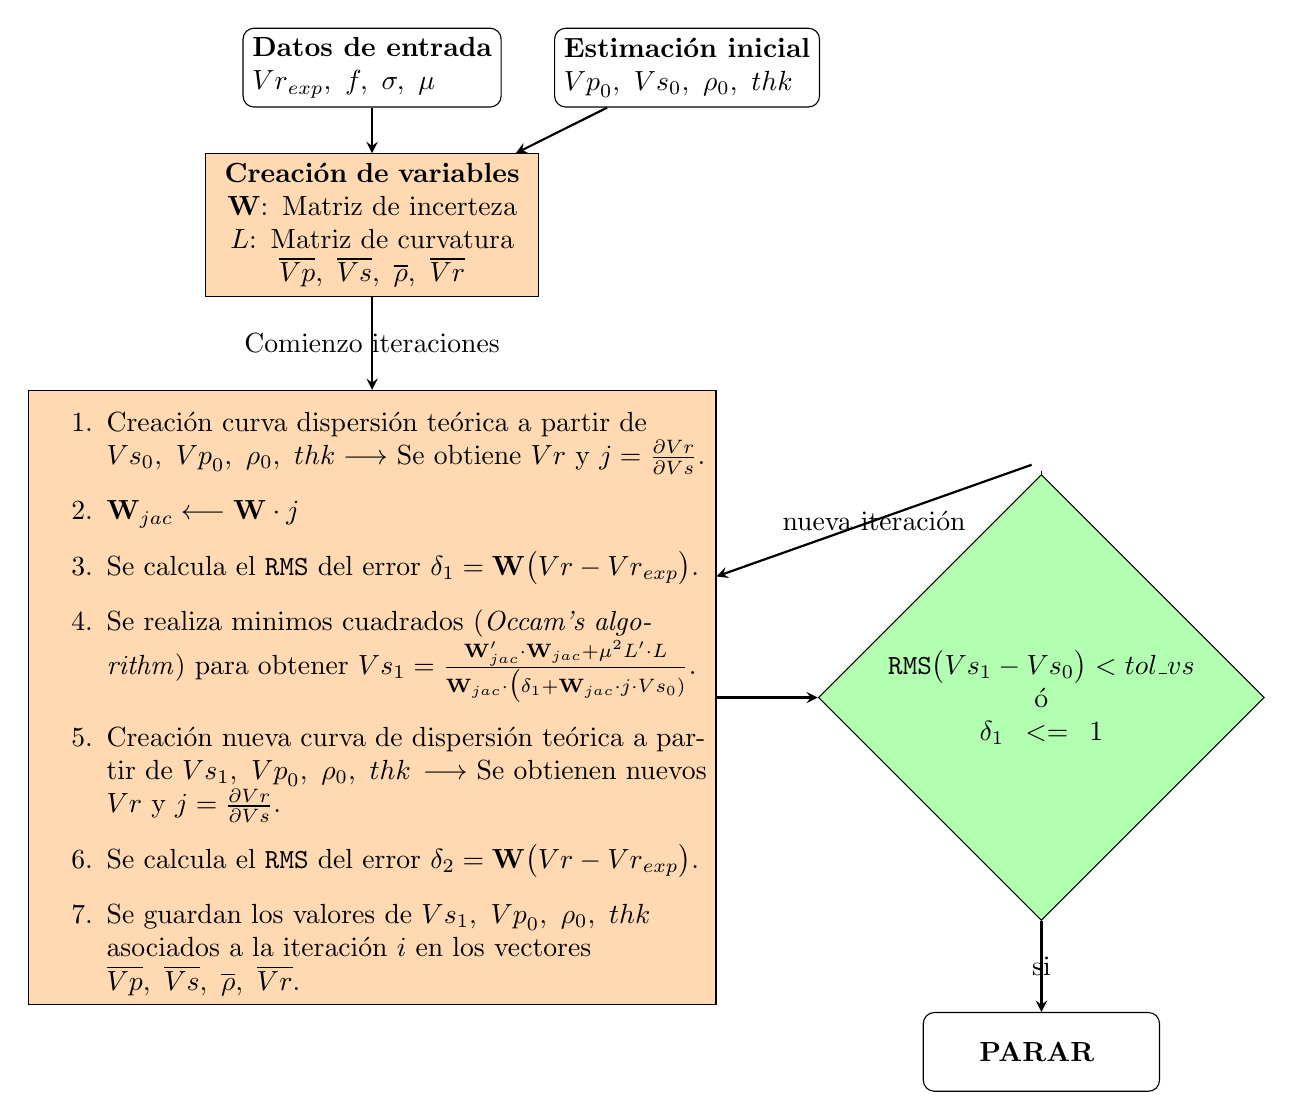
\begin{tikzpicture}
		\node (ent1) [startstop, align=left] {
			\textbf{Datos de entrada}\\
			$\lpow{Vr}{exp},\ f,\ \sigma,\ \mu$
		};
		\node (ent2) [startstop, right of=ent1, xshift=3cm, align=left] {
			\textbf{Estimación inicial}\\
			$\lpow{Vp}{0},\ \lpow{Vs}{0},\ \lpow{\rho}{0},\ thk$
		};
		\node (creacion) [process, below of=ent1, yshift=-1.cm, xshift=0cm, text width=4cm] {
			\textbf{Creación de variables}\\
			${\bf W}$: Matriz de incerteza\\
			$L$: Matriz de curvatura\\
			$\overline{Vp},\ \overline{Vs},\ \overline{\rho},\ \overline{Vr}$ 
		};
		\node (iteracion1) [process, below of=creacion, yshift=-5cm, text width=8.5cm] {
			\vspace{-0.3cm}
			\begin{enumerate}
			\item Creación curva dispersión teórica a partir de $\lpow{Vs}{0},\ \lpow{Vp}{0},\ \lpow{\rho}{0},\ thk \longrightarrow$ Se obtiene $Vr$ y $j=\fracpartial{Vr}{Vs}$.
			\item ${\bf W}_{jac} \longleftarrow {\bf W}\cdot j$
			\item Se calcula el \texttt{RMS} del error $\delta_1 = {\bf W}\big(Vr - \lpow{Vr}{exp}\big)$.
			\item Se realiza minimos cuadrados (\textit{Occam's algorithm}) para obtener $\lpow{Vs}{1} = \frac{{\bf W}_{jac}'\cdot {\bf W}_{jac} + \pow{\mu}{2}L' \cdot L}{{\bf W}_{jac} \cdot \big(\delta_1 + {\bf W}_{jac} \cdot j\cdot \lpow{Vs}{0})}$.
			\item Creación nueva curva de dispersión teórica a partir de $\lpow{Vs}{1},\ \lpow{Vp}{0},\ \lpow{\rho}{0},\ thk \longrightarrow$ Se obtienen nuevos $Vr$ y $j=\fracpartial{Vr}{Vs}$.
			\item Se calcula el \texttt{RMS} del error $\delta_2 = {\bf W}\big(Vr - \lpow{Vr}{exp}\big)$.
			\item Se guardan los valores de $\lpow{Vs}{1},\ \lpow{Vp}{0},\ \lpow{\rho}{0},\ thk$ asociados a la iteración $i$ en los vectores $\overline{Vp},\ \overline{Vs},\ \overline{\rho},\ \overline{Vr}$.
			\end{enumerate}
		};
		\node (decision1) [decision, right of=iteracion1, text width=4cm, xshift=7.5cm, yshift=0cm] {
			$\texttt{RMS} \big(\lpow{Vs}{1}-\lpow{Vs}{0}\big) < tol\_vs$ \\ó\\
			$\delta_1 <= 1$
		};
		\node (end1) [startstop, align=left, below of=decision1, yshift=-3.5cm] {
			\textbf{PARAR}
		};
		\node (conector1) [above of=decision1, yshift=2cm, text width=0cm]{};
		\draw [arrow] (ent1) -- (creacion);
		\draw [arrow] (ent2) -- (creacion);
		\draw [arrow] (creacion) -- node {Comienzo iteraciones} (iteracion1);
		\draw [arrow] (iteracion1) -- (decision1);
		\draw [arrow] (decision1) --node {si} (end1);
		\draw  (decision1) -- (conector1);
		\draw [arrow, xshift=3cm] (conector1) --node {nueva iteración} (iteracion1);
	\end{tikzpicture}
\end{document}